\documentclass[11pt,a4paper]{scrartcl}
\setlength{\parindent}{0pt}
\setlength{\parskip}{5pt}

\newcounter{mycommentcounter}
\newcommand{\Genericcomment}[2]{%
\par%
\noindent%
\fbox{%
\begin{minipage}{0.95\textwidth}
\textsl{#1: \#\refstepcounter{mycommentcounter}%
\arabic{mycommentcounter}: #2}%
\end{minipage}%
}%
\par%
}

\newcommand{\AVTcomment}[1]{
\Genericcomment{AVT}{#1}
}

\newcommand{\SKcomment}[1]{
\Genericcomment{SK}{#1}
}

\newcommand{\HashValue}[0]{\mathsf{HashValue}}
\newcommand{\Mask}[0]{\mathsf{Mask}}
\newcommand{\XOR}[0]{\mathtt{XOR}}
\newcommand{\AND}[0]{\mathtt{AND}}
\newcommand{\rol}[0]{\mathtt{rol}}
\newcommand{\ror}[0]{\mathtt{ror}}

\usepackage{amsmath}
\usepackage{amsfonts}
\usepackage{mathtools}
\usepackage{graphicx}
\usepackage{pdfpages}
\usepackage{algpseudocode}
\usepackage{algorithm}
\usepackage{palatino}
\usepackage{numprint}
\usepackage{svg}
\usepackage[colorlinks=true, allcolors=blue]{hyperref}
\title{Efficient Preprocessing of Short Sequence Segments for Efficient Filtering in Comparing Protein Sequences}
\author{Anh Viet Ta (6747004)}

\begin{document}
\begin{titlepage}
\maketitle
\pagenumbering{gobble}% Remove page numbers (and reset to 1)
\thispagestyle{empty}

\textbf{Abstract:} 
\end{titlepage}
\pagenumbering{arabic}
\setcounter{page}{1}

\section{Introduction}
\section{MMseqs2}
\subsection{Introduction}
\subsection{Fast q-gram prefiltering stage}
\subsection{Ungapped alignment stage}
\subsection{Smith-Waterman alignment stage}
\section{Theory}
\subsection{Algorithm description}
Given a residue alphabet \(\Alpha\) and
\(\sigma:\Alpha\times\Alpha\to\Reals\)  a score function. For
\(u,v\in\Alpha^{\ast}\), \(|u|=|v|\) is the score defined as

$$\sigma(u,v)=\sum_{i=0}^{|u|-1}\sigma(\Subchar{u}{i},\Subchar{v}{i})$$

In order to compute the $k$-environment for a \(7\)-gram efficiently, we decompose it to one group of trigram and two groups of digrams, for all of which a primary environment \(\Scoretable{u}=\lbrack (v,\sigma(u,v))\mid v\in\Alpha^{q}\rbrack\) is computed and sorted after the subscores \(\sigma(u,v))\).

The full $k$-environment of the \(7\)-gram can then be iterated as the cartesian product
\begin{align}
\Scoretable{\Substring{u}{0}{2}}\times \Scoretable{\Substring{u}{3}{4}}\times
\Scoretable{\Substring{u}{5}{6}}\label{ScoreTablesCartesian}
\end{align}
The iteration over primary environments can then stop, when it's no longer feasible to reach the threshold \(k\).

The key to improve over the method outlined in MMseqs2, is the following:

Given a bijective mapping \(\varphi:\{0,1,\ldots,q-1\}\to \{0,1,\ldots,q-1\}\). For any sequence of length \(q\),  we define a function
\begin{align}
\varphi(u)=\Subchar{u}{\varphi(0)}\Subchar{u}{\varphi(1)}\ldots\Subchar{u}{\varphi(q-1)}  
\end{align}
in that, \ \(\varphi\) permutate the residue in \(u\).

Given a special permutation \(\Permname{u}\), so that it orders the characters in \(u\): \(\Subchar{u}{\Perm{u}{i}}\leq\Subchar{u}{\Perm{u}{i+1}}\forall i, 0\leq i\leq q-2\). The resulted \(q\)-gram \(u_s\) from the permutation is then sorted \(q\)-gram and could be rearranged using the inverse function:
\begin{align}
\Perminverse{u}{\Perm{u}{i}}=i \forall i, 0\leq i\leq q-1 \Rightleftarrow \Perminverse{u}{\Perm{u}{u}}=u
\end{align}

It can be shown that
\begin{align}
\sigma(u,v)=\sigma(\Perm{u}{u},\Perm{u}{v}) \forall v\in\Alpha^{q}
\end{align}
which means, the same permutation function applied on both sequences \(u\) and \(v\)
permutates the characters in the same way and the score between the unpermutated sequences is equal to the score between the permutated. This means that the score matrix ST can be computed only for the sorted \(q\)-grams, and it would hold all scores needed to compute the full $k$-environment.

The advantage of this approach is the smaller number of sorted $q$-grams compared to unsorted, leading to a more efficient memory usage and a more compacted computation of the score matrix ST. Any overhead caused by the rearragement of the sorted $q$-grams, see Equation~\ref{Scoretableuprime}, can be reduced by SIMD instructions.
\subsection{Sorted and unsorted q-grams}
\section{Implementation \& Design}
\subsection{Input}
At compile time, the program takes in a scoring function, which in the context of protein sequences could be a BLOSUM or PAM matrix, a spaced seed and a recursive hashing function. The scoring function should detail the relevant alphabet, the transformer function, which encodes every character in the alphabet to its corresponding rank, and a matrix of scores between every pairs of characters. Internally, the spaced seed is initially represented as a numeric constant, which during computation will be transcoded into a bitset. The span of the seed can then be computed according to the position of the first 1 in the bitset and also the seed weight can be calculated by counting 1s. 

At run time the program takes in two sequence databases in FASTA format. Any data error, for example empty file or wrong data format will automatically lead to termination of the program and an error message will be logged. Additionally, the sensitivity of the program can be adjusted.

To further assist in expansion, some fixed parameters, e.g maximum sub-$q$-gram length are defined as preprocessor constants.
\subsection{Structure}
\subsubsection{Relevant classes and dataflow}
The program consists of six main classes:
\begin{enumerate}
    \item SortedQgram, which creates a table to index every sorted q-gram of given $ScoreClass$ and $q$.
    \item MultisetEncoder, which creates a table to encode every possible sorted q-gram to integer.
    \item Distribution, which approximates a threshold $k$ for a $k$-environment given a $ScoreClass$.
    \item QgramEnvironment, which generates a score matrix between all sorted $q$-grams and unsorted $q$-grams.
    \item SpacedSeedEncoder, which generate schemes to divide spaced seed, divides them into sub-$q$-grams and encodes them into sorted $q$-gram codes.
    \item CompositeEnvironment, which is the main class. It passes sequences into SpacedSeedEncoder, uses the sorted $q$-gram codes to call individual $k$-environment and generates a Cartesian product from the environments.
\end{enumerate}
In Figure~\ref{fig:classes}, the relationship and dataflow between the classes are outlined.

\begin{figure}[t]
\begin{center}
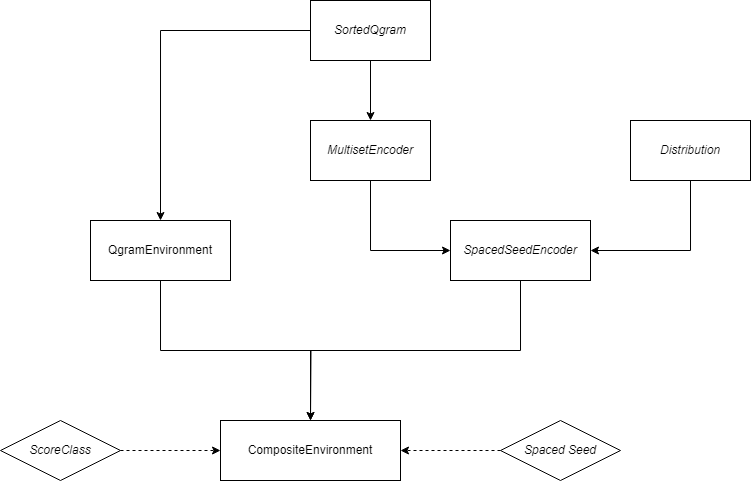
\includegraphics[scale=0.6]{graphics/Class Diagram.png}
\end{center}
\caption{Relationship between the six main classes and inputs. $Italic$ denotes compile-time evaluated classes.}
\label{fig:classes}
\end{figure}
\subsubsection{Datatypes}
\input{Implementation_structure_datatypes}
\subsection{Approximating threshold}
In MMseqs, in order to evaluate a proper threshold \(k\) for the environment, a \(z\)-score statistics was applied. For each query sequence, a calibration search through a subset of 100~000 randomly sampled target sequences is performed, where the number of prefiltering operations
\begin{align}
    \text{sum}_L = \sum_{t=1}^{100~000} (L_t-k+1)
\end{align}
and its sum of scores
\begin{align}
    \text{sum}_S = \sum_{t=1}^{100~000} S_{qt}
\end{align}
are recorded. \(L_t\) here denotes the length of the target sequence \(t\) and \(S_{qt}\) the prefiltering score between query sequence \(s\) and target sequence \(t\). The expected chance prefiltering score between them is then
\begin{align}
    S_0 = (L_t-k+1)\frac{\text{sum}_S}{\text{sum}_L}
\end{align}
Assuming the number of \(q\)-gram matches is Poisson-distributed, the standard deviation of the scores \(\sigma_S\) can be computed through number of expected \(q\)-gram matches \(n_{\text{match}}\):
\begin{align}
    n_{\text{match}} &\approx \frac{S_0}{S_{\text{match}}}
\end{align}
\begin{align}
    \sigma_S &= S_{\text{match}}\sqrt{n_{\text{match}}}\\
    &= \sqrt{(L_t-k+1)\frac{\text{sum}_S}{\text{sum}_L}S_{\text{match}}}
\end{align}
where \(S_{\text{match}}\) is the expected score per chance \(q\)-gram match. The significant prefiltering score \(S_{qt}\) should then fulfill the condition
\begin{align}
    S_{qt} \geq Z_{thr}\sigma_S + S_0
\end{align}
where \(Z_{thr}\) is the significant \(z\)-score. MMseqs2 would take in a sensitivity parameter \(s\), labeled internally as the average length of \(q\)-gram list each sequence position, from the user and using a heuristic to compute for \(S_{qt}\). This approach is shown to be lacking in control for \(s\) and therefore the goal is to streamline the process and to allow for a more fine-grained control of the length of \(q\)-gram list. 

In order to approximate an appropriate threshold \(k\) for a \(q\)-gram environment, a distribution of pairwise amino acid scores is generated. This distribution is then convoluted with itself \(q-1\) times to create a distribution of unsorted-$q$-grams-vs-unsorted-$q$-grams score and the threshold can be then obtained by filtering only a fraction of the top scores. This approach could then be easily adapted for any given target amino acid distribution, where the expected probability of the \(q\)-grams is integrated into the distribution of the pairwise amino acid scores. %But since the evaluting scheme demands a score distribution between sorted and unsorted \(q\)-grams

\subsection{Sorted q-grams}
\subsubsection{Enumeration}
In mathematics, a set is defined as a collection of items, where every element occurs exactly once. This definition can be expanded to multisets, where elements can occur more than once. Applying an order on these multisets, we can formalize a notion of sorted \(q\)-grams:

Given an alphabet \(\Alpha\) and a natural number \(q > 0\), a sorted \(q\)-gram over \(\Alpha\) is a multiset \(M=a_0a_1...a_{q-1}\), \(a_i\in\mathcal{A}\forall 0\leq i<q\) and \(a_i \leq a_j\forall 0\leq i < j < q\).

%The number of possible sorted \(q\)-grams for a given \(\mathcal(A)\) and \(q\) can be computed as the binomial \(\binom{q+|\mathcal{A}|-1}{q}\). The proof can be shown with induction: 
An index table of sorted \(q\)-grams can be computed recursively. Given a sorted \(q\)-gram \(u\) where the prefix of \(m\) characters is sorted and fixed, and \(u[m-1]\) has a rank of \(a_i\) then the task is to enumerate every \((q-m)\)-grams of alphabet size (\(|\mathcal{A}|-a_i\)). The induction base case is then sorted unigrams over alphabet \(\Alpha_i = \{a_j| a_j\in\Alpha \land j\geq i\}\), where there are \(|\Alpha_i|\) unigrams indexed from \(a_i\) to \(|\Alpha|-1\).

\begin{algorithm}[t]
\caption{multisetEnumerateRecursion}
\label{code:enumerateMultisetRec}
\begin{tabular}{@{}l@{~}l}
\textbf{Input:}&current multiset length \(q\)\\
               &current alphabet \(\Alpha_i\)\\
               &current prefix \(u\)\\
               &current index table IT\\
\end{tabular}
\begin{algorithmic}
\If{\(q = 0\)}
\State \(\text{IT.append}(u)\)
\Else
\For{\(a_j \in \Alpha_i\)}
\State \(multisetEnumerateRecursion(q-1,\Alpha_i \backslash [a_i,a_j),u+a_j,\text{IT})\)
\EndFor
\EndIf
\end{algorithmic}
\end{algorithm}

\begin{algorithm}[t]
\caption{multisetEnumerate}
\label{code:enumerateMultiset}
\begin{tabular}{@{}l@{~}l}
\textbf{Input:}&multiset length \(q\)\\
               &alphabet \(\Alpha\)
\end{tabular}
\begin{algorithmic}
\State \(\text{IT}\gets []\)
\For{\(a_i \in \Alpha\)}
\State \(multisetEnumerateRecursion(q-1,\Alpha \backslash [a_0,a_j),a_i,\text{IT})\)
\EndFor
\end{algorithmic}
\end{algorithm}

\subsubsection{Linear encoding}

Using the index table, a scheme to encode any given \(q\)-gram over alphabet \(\Alpha\) to its table index in \(O(q)\) can be devised. The proposition is, there exists an unique integer weight for each character \(a\) in position \(p\) so that given any sorted \(q\)-gram \(u\) over an alphabet \(\Alpha\),
\begin{align}
    c(u)=\sum_{p=0}^{q-1} w(p,u[p])\label{Equation:linearenc}
\end{align} 

encodes exactly \(u\) to its index in table IT. This can be shown with induction:

\textbf{Base case:} In case of \(q=1\), \(|\Alpha|\) unigrams can be clearly encoded with \(w(0,a) = a \forall a \in \Alpha\).

\textbf{Inductive step:} Given the above scheme is valid up until \(q\in \mathcal{N}\), it needs to be shown \(w(q,a)\) is unique for all \(a\in \Alpha\). Assuming the weight isn't unique, therefore there exist two different weights \(w_a\neq w_a'\) so that \(c(au) = w_a + c(u)\) and \(c(av) = w_a' + c(v)\) encode \((q+1)\)-grams \(au\) and \(av\) respectively, \(u,v\in \Alpha^q,a\in\Alpha\). The codes \(c(au)\) and \(c(av)\) must but differ exactly the code of their suffixes \(c(u)-c(v)\), since the \(q+1\)-grams share the same prefix. One can then formulate:
\begin{align}
    c(au) - c(av) &= (w_a + c(u)) - (w_a' + c(v))\\
    &= (w_a - w_a') + (c(u) - c(v))\\
    &= c(u) - c(v)
\end{align}
which leads to \(w_a - w_a' = 0\), or \(w_a = w_a'\), which is a contradiction.

The recursive method to then compute a \(q\times |\Alpha|\) table LE is based on the above proof. The base case can be directly given and based on index tables \(\text{IT}_{q_i,\Alpha},2 \leq q_i \leq q\), the \(q_i\)-grams are tracked for change in prefix and the weight of the prefix can be calculated with Equation~\ref{Equation:linearenc}.
\begin{algorithm}[t]
\caption{Creating linear encoding table}
\label{code:linearEncodingTable}
\begin{tabular}{@{}l@{~}l}
\textbf{Input:}&sequence length \(q\)\\
               &alphabet \(\Alpha\)\\
               &index tables \(\text{IT}_{q_i,\Alpha}\forall q_i \in [1,q]\)\\
\end{tabular}
\begin{algorithmic}
\State LE \(\gets []\)
\State LE.append(\([0,...,|\Alpha|-1]\))
\For{\(q_i\in[2,q]\)}
\State \(\CurrentWeight \gets [None \times |\Alpha|]\)
\For{\(u,i\in\text{IT}_{q_i,\Alpha}\)}\Comment{Key-Value loop}
\If{\(\CurrentWeight [u[0]] = None\)}
\State \(\SuffixCode\gets 0\)
\For{\(j \in [1,q_i]\)}
\State \(\SuffixCode += \text{LE}[j-1][u[j]]\)
\EndFor
\State \(\CurrentWeight [u[0]] \gets i - \SuffixCode\)
\EndIf
\EndFor
\State \(\text{LE}.insert(0,\CurrentWeight)\)\Comment{Place more significant weight at beginning}
\EndFor
\end{algorithmic}
\end{algorithm}

\begin{comment}
\begin{algorithm}[t]
\caption{Linear encoding of sorted \(q\)-grams}
\label{code:linearEncode}
\begin{tabular}{@{}l@{~}l}
\textbf{Input:}&sorted \(q\)-gram \(u\)\\
                &alphabet \(\Alpha\)\\
               &linear encoding table LE of size \(q\times|\Alpha|\)
\end{tabular}
\begin{algorithmic}
\State \(\text{Code} \gets 0\)
\For{\(i\in [0,q-1]\)}
\State \(\text{Code} += \text{LE}[i][u[i]]\)
\EndFor
\State return \(\text{Code}\)
\end{algorithmic}
\end{algorithm}    
\end{comment}

\subsubsection{Enumerating}
\subsubsection{Encoding sequence in linear time}
\subsection{Extracting and sorting q-gram from spaced seeds}
Internally the spaced seed is stored and represented as a 64-bit constant integer. The first step to process this spaced seed is a conversion to a bitset. Its span could then be determined as the length of the bitset subtracted by the position of the most significant 1-bit and its weight is then obtained by iterating over its span.

The program also creates a scheme to divide the spaced seed. The position of the heavier primary environments (if any) is placed at the earlier portion of the spaced seed.

In order to prepare for the recursive hashing of the target sequences, the spaced seeds are also divided in $b$ blocks of smaller $q$-grams. The complexity of the recursive hashing of a sequence of length $n$ is $O(nb)$.
\subsection{Constructing sub-q-gram environments}
\input{Implementation_constructing}
\subsection{Iterating over sequence}
In the implementation of MMseqs2, a mechanism to evaluate the surrounding of current position while iterating the query sequences is introduced. The idea of this mechanism is to adjust the threshold of the \(q\)-gram environment in response to regions where local composition varies considerably from the background distribution. Without adjusting, these low regions can lead to biases in the prefiltering result. This correction of the threshold can be summarized as follow:
\begin{align}
    \Delta S_i(u[i]) = \sum_{a=1}^{|\mathcal{A}|}f(a)\sigma(a,u[i])-\frac{1}{2d}\sum_{j=i-d,j\neq i}^{i+d}\sigma (u[i],u[j])
\end{align}
where \(u\) is the query sequence, \(i\) the current residue on the sequence and \(f(a)\) the background frequency of residue \(a\).

The minuend is a representation of the expected score resulting from the background distribution, which can be precomputed when the target data is read. The subtrahend involves the current region in the query sequence and introduces a parameter \(d\) for the radius of the region, defined in MMseqs2 as a constant 20.

The corrected score can then be computed as the sum of the pairwise amino acid score and the score correction. In the implementation, this correction is subtracted from the threshold at the beginning of the computation.

An issue in enumerating the Cartesian product is the possible difference in number of loops (e.g 2 loops for seed weight 4-6, 3 loops for seed weight 7). To resolve this problem and allow the easy expansion to greater seed size, a flexible loop structure is designed, where an array containing the loop indexes is created. The earliest entry of the array holds the most outer loop index and the later an entry is, the more inner the loop index the entry holds. By iterating through only the most outer loop and only adjusting the inner loop indexes as needed, the scheme can account for any number of loops.

The formulation of the loop structure, along with the integration of background score correction, is outlined in the pseudocode below:

\begin{comment}
\begin{algorithm}[t]
\caption{Merging query and target data}
\label{code:merging_data}
\begin{tabular}{@{}l@{~}l}
\textbf{Input:}&query data \(query\)\\
               &target data \(target\)
\end{tabular}
\begin{algorithmic}
\For{\(i\) \textbf{from} 1 to $|\mathcal{A}|$} \Comment{Generate random
integers for each character}
\State \(f(A[i]) \gets \mathsf{RandomInteger}()\)
\EndFor
\For{\(i\) \textbf{from} 1 to $|\mathcal{A}|$} \Comment{Generate lookup
table to remove character}
\State \(f_r(A[i]) \gets \rol(f(A[i]),k-1)\)
\EndFor
\State \(\HashValue \gets 0\)
\For{\(i\) \textbf{from} 1 to $k$} \Comment{Compute first hash value}
\State \(\HashValue = \rol(\HashValue,1)\)
\State \(\HashValue = \XOR(\HashValue,f(s[i]))\)
\EndFor
\State \(\mathsf{process}(\HashValue)\)
\For{\(j\) \textbf{from} 1 to $n-k$} \Comment{Compute other hash values}
\State \(\HashValue = \XOR(\HashValue,\rol(f(s[j]),k-1))\)
\State \(\HashValue = \rol(\HashValue,1)\)
\State \(\HashValue = \XOR(\HashValue,f(s[j+k])\)
\State \(\mathsf{process}(\HashValue)\)
\EndFor
\end{algorithmic}
\end{algorithm}
\end{comment}

\subsection{SIMD}
The key to the shuffle using SIMD is the instruction \_\_mm\_shuffle\_epi8, which is available on platforms supporting SSSE3 instruction sets. The instruction takes in two 128-bit (equivalent to 16-byte) vectors, first vector holds the data, and the second the information on how the data get shuffled. A schematic can be seen below:

When the program is opted to process the q-grams with SIMD, the unshuffled q-grams are first packed as-is. After every valid elements are in the result vector, the function shuffle\_with\_simd is called, which looks up every to-be-shuffled element, starting from the end of vector. The q-grams, which individually takes up $q$ bytes each, are then packed as much as possible on a 128-bit (equivalent to 16-byte) vector called $buf$ according to the following expression:

$$\text{num\_per\_vector} = \frac{16}{q}$$

Along with vector $buf$, another vector is created, which holds information on permutation. After the two vectors are set up, the instruction \_\_mm\_shuffle\_epi8 is called and the shuffled q-grams then get extracted and replace the unshuffled in the result vector.
\subsection{Output}
After being collected, the hashed data from the target and query sequences are packaged as byte units, prioritizing hash values. They then get sorted individually using radix sort (see GTTL), resulting in two data vectors sorted by hash values which would then be merged value by value, skipping through unmatching blocks.

\begin{algorithm}[t]
\caption{Merging query and target data}
\label{code:merging_data}
\begin{tabular}{@{}l@{~}l}
\textbf{Input:}&query data \(query\)\\
               &target data \(target\)
\end{tabular}
\begin{algorithmic}
\State \(target\_idx \gets target.start\)
\State \(query\_idx \gets target.start\)
\While{\(target\_idx \neq target.end\) \(\land\) \(query\_idx \neq query.end\)}
\State \(target\_hashval \gets target[target\_idx].hashval\)
\State \(query\_hashval \gets query[query\_idx].hashval\)
\If{\(target\_hashval < query\_hashval\)} \Comment{Skipping on target vector}
\While{\(target[target\_idx].hashval = target\_hashval\)} 
\State \(target\_idx++\)
\EndWhile
\Else
\If{\(target\_hashval > query\_hashval\)} \Comment{Skipping on query vector}
\While{\(query[query\_idx].hashval\)} 
\State \(query\_idx++\)
\EndWhile
\Else \Comment{Match found}
\State \(target\_block\_end = target\_idx\) 
\While{\(target[target\_block\_end] = target\_hashval\)}
\State \(target\_block\_end++\)
\EndWhile
\State \(query\_block\_end = query\_idx\)
\While{\(query[query\_block\_end] = query\_hashval\)}
\State \(query\_block\_end++\)
\EndWhile
\State \(create\_matches([target\_idx,target\_block\_end),[query\_idx,query\_block\_end))\)
\EndIf
\EndIf
\EndWhile
\end{algorithmic}
\end{algorithm}

The merging process results in a vector of matches, represented again as byte units, containing respectively the sequence number of the match on the target, on the query, the diagonal number (difference between the target and query sequence position), and the query sequence position. These quartets are again sorted with radix sort to prepare for ungapped alignment stage.
\section{Benchmark \& Performance}
\subsection{Time performance}
\subsubsection{Compile time performance}
\subsubsection{Execute time performance analysis with gprof}
\subsubsection{Dependence of execute time on acceptance rate}
\subsection{Spatial Performance with valgrind massif}
\section{Retrospection \& Future improvements}
\subsection{Scalability}
\subsection{Full compile-time calculation of environments}
\section{Conclusion}
\section{Reference}

\end{document}
